%% appendix_seasonal.tex — Seasonal sensitivity of P(H) within the Cassini window
%% DRAFT: summary of the exploratory half-Titan-year seasonal analysis.

\chapter{Seasonal Sensitivity Within the Cassini Window}
\label{app:seasonal}

The five-epoch reconstruction of Chapter~\ref{ch:methods} treats the
\textit{Present} as a single time-averaged state.  The Cassini dataset,
however, spans 2004--2017: about $0.44$ of a Titan year (the Titan year being
$29.46$\,yr), running from a mid-southern season through the northern spring
equinox in 2009.61 and reaching the northern summer solstice only at the very
end of the mission.  This appendix summarises an exploratory analysis of how
far the posterior moves across that half-year window.  The headline conclusion
is that the framework \emph{can} be pushed to a seasonal question, but only
with substantial caveats: of the eight features, only one carries any seasonal
signal at all, and the temperature model available for that feature is valid
only over the mission window.

\section{Which Features Vary}
\label{sec:seasonal_which}

Only the methane cycle feature $f_4$ has a time-dependent component.  It is
the weighted composite
\[
  f_4 = 0.50\,g_T + 0.35\,d_c + 0.15\,p_\phi,
\]
where $g_T$ is the normalised CIRS meridional temperature gradient
$|\partial T/\partial\,\mathrm{lat}|$, $d_c$ the fluvial channel density, and
$p_\phi$ the latitude prior centred on $\pm 50\textdegree$.  Of these, only the
temperature-gradient term $g_T$ varies in time; the channel density and
latitude prior are static.  The other seven features derive from
time-averaged mosaics or from quantities (terrain class, topography, interior
structure) that do not vary on seasonal timescales, so they are seasonally
invariant here by construction or by physics.  The seasonal temperature field
is taken from the model of \citet{Jennings2019}, a cosine in latitude whose
parameters vary linearly in year ($a + bY$, with $Y = \text{year} - 2009.61$
centred on the equinox), fit to CIRS observations and stated by its authors to
be valid only over $Y \in [-4.9, +8.1]$.  Propagating a change in $f_4$
through the Bayesian update shifts the posterior by
\[
  \Delta P(H) = \frac{\lambda w_4}{\kappa + \lambda}\,\Delta f_4
  = 0.0818\,\Delta f_4,
\]
so even a large swing in $f_4$ produces only a small posterior shift,
consistent with the feature's Tier-2 weight ($w_4 = 0.15$).

\section{What Was Found}
\label{sec:seasonal_found}

Sweeping the \citet{Jennings2019} temperature term across 2004--2017 while
holding all other features fixed produces a modest, one-directional modulation
of the posterior, concentrated at northern high latitudes
(Figure~\ref{fig:seasonal_ph_app}).  The zonally-averaged northern polar band
falls from $0.404$ to $0.368$ and the northern mid-latitude band from $0.367$
to $0.337$; the top-10 present-epoch sites (all north polar lakes) decline by
$\sim$0.035 in $P(H)$ (Towada Lacus, for example, from $\sim$0.59 to
$\sim$0.56).  The equatorial and southern bands are essentially flat (changes
$\leq 0.01$), the southern bands showing only a shallow maximum just after
equinox.  The decline reflects the meridional temperature gradient flattening
as the northern hemisphere moves from winter towards summer, weakening the
gradient-based methane-cycle proxy at the very latitudes where the
highest-scoring lakes sit.  The amplitude ($\leq 0.04$ in $P(H)$) is small in
absolute terms and well within the $\sim$0.5 width of the posterior credible
intervals, so it does not alter any site ranking; its interest is as a
directional, physically interpretable trend rather than a change in the
habitability conclusions.

\begin{figure}[H]
  \centering
  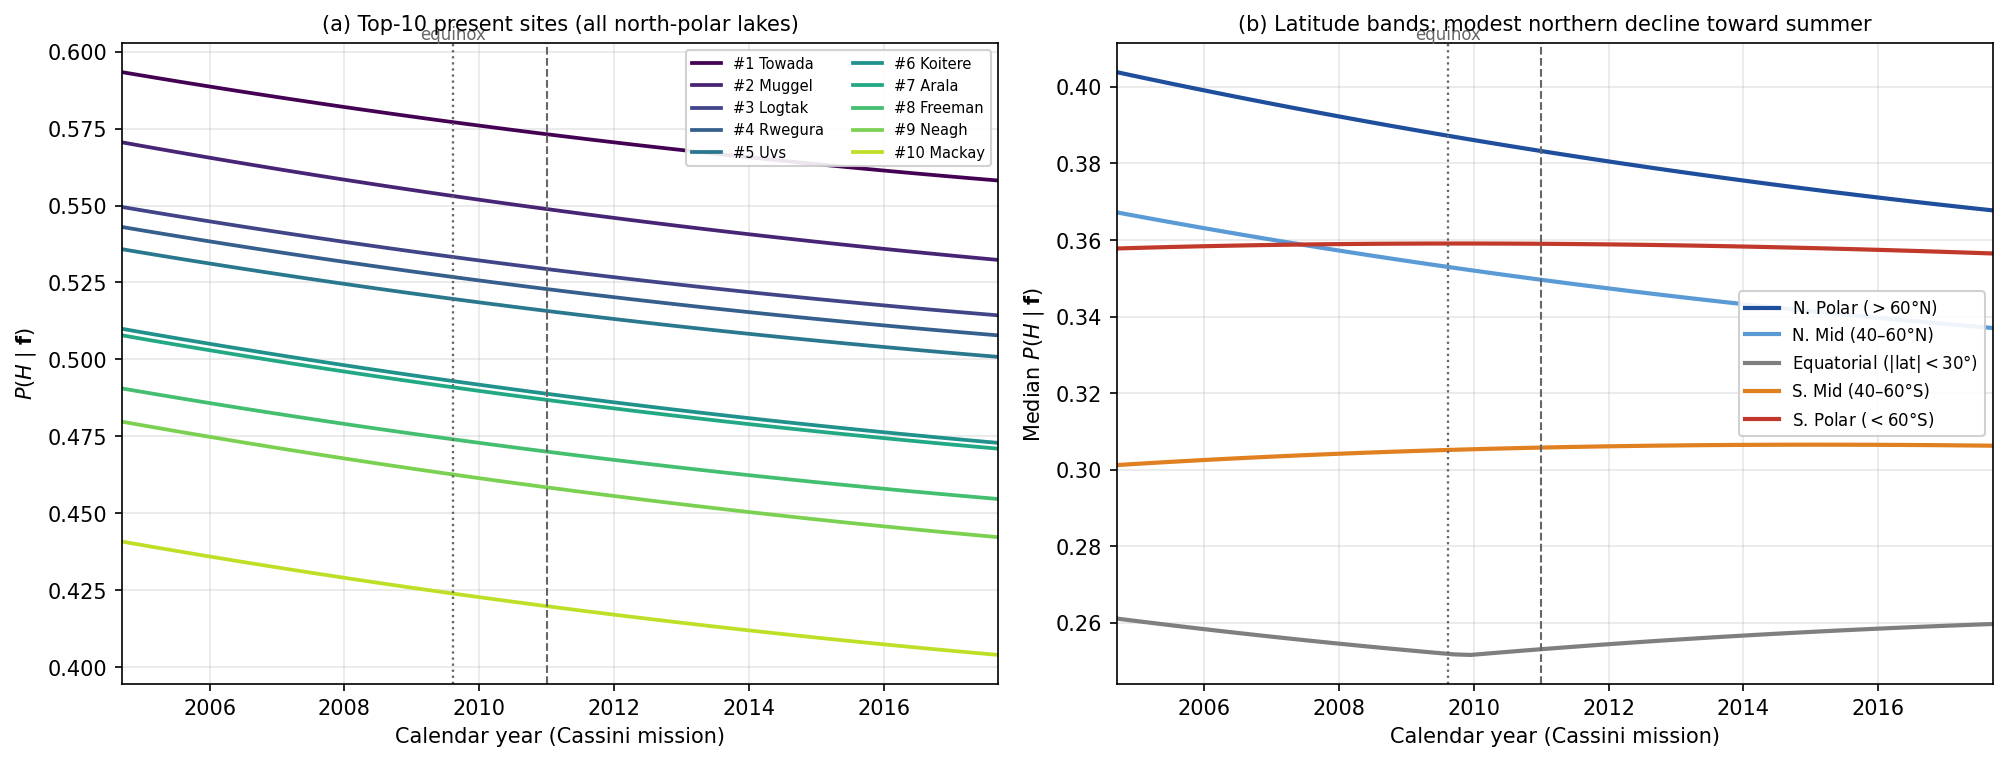
\includegraphics[width=\textwidth]{images/seasonal_ph_trend.png}
  \caption{Seasonal modulation of the posterior $P(H \mid \featurevec)$ across
    the Cassini window (2004--2017), computed by sweeping the
    \citet{Jennings2019} meridional-temperature term of the methane cycle
    feature ($f_4$) while holding the other seven features fixed.  (a)~The
    top-10 north-polar lake sites each fall by $\sim$0.035 (e.g.\ Towada Lacus
    $\sim$0.59 to $\sim$0.56).  (b)~By latitude band, the northern polar band
    declines from $0.404$ to $0.368$ and the northern mid-latitude band from
    $0.367$ to $0.337$, while the equatorial and southern bands remain flat
    ($\leq 0.01$, the southern bands showing only a shallow post-equinox
    maximum).  The decline is the pre-solstice flank of a cycle, not a
    symmetric hemispheric reversal.}
  \label{fig:seasonal_ph_app}
\end{figure}

\section{Limitations and a Periodic Extension}
\label{sec:seasonal_limits}

Two limitations should be stated plainly.  First, the $f_4$ proxy rewards the
meridional temperature gradient that drives large-scale transport (steepest
towards winter), not the convective activity that peaks in summer; the signal
it reports is a gradient-transport signal, and it is zonal (latitude-only).
Second, the \citet{Jennings2019} field is a cosine in latitude whose peak
tracks the \emph{subsolar latitude} (the latitude lying directly beneath the
Sun, which migrates north and south over a Titan year and drives the seasons);
the model has that peak advance linearly in year.  This captures the
latitudinal temperature profile and its drift across the observed half-window,
but a linear march is only a local approximation and cannot represent a full
seasonal cycle: it moves the subsolar latitude at about $3.2\textdegree$ per
year, which over a full Titan year (29.46\,yr) would carry it through
$\sim$94\textdegree.  The subsolar latitude cannot in fact travel that far,
because Titan's axial tilt (its \emph{obliquity}, $26.7\textdegree$) confines
it to the band $\pm 26.7\textdegree$, within which it oscillates and reverses
direction at each solstice.  The linear fit is therefore valid only inside the
mission window: extrapolated further it would drive the subsolar point past
this physical limit, and it cannot reproduce the solstice turnover (the moment
at which the subsolar latitude reaches $\pm 26.7\textdegree$ and the seasonal
trend reverses).

Substituting the true astronomical subsolar latitude,
$26.7\textdegree \cdot \sin\!\big(2\pi(\text{year}-2009.61)/29.46\big)$, into
the same cosine form (with amplitude and contrast held at their equinox values
rather than re-fit) agrees with the \citet{Jennings2019} model inside the
observed window but rolls over at the 2017 solstice and is bounded and
periodic (Figure~\ref{fig:seasonal_periodic_app}).  This confirms that the
decline above is the pre-solstice flank of a bounded cycle rather than an
unbounded trend.  The periodic form is illustrative only: it is not re-fit to
data and has not been validated.

\begin{figure}[H]
  \centering
  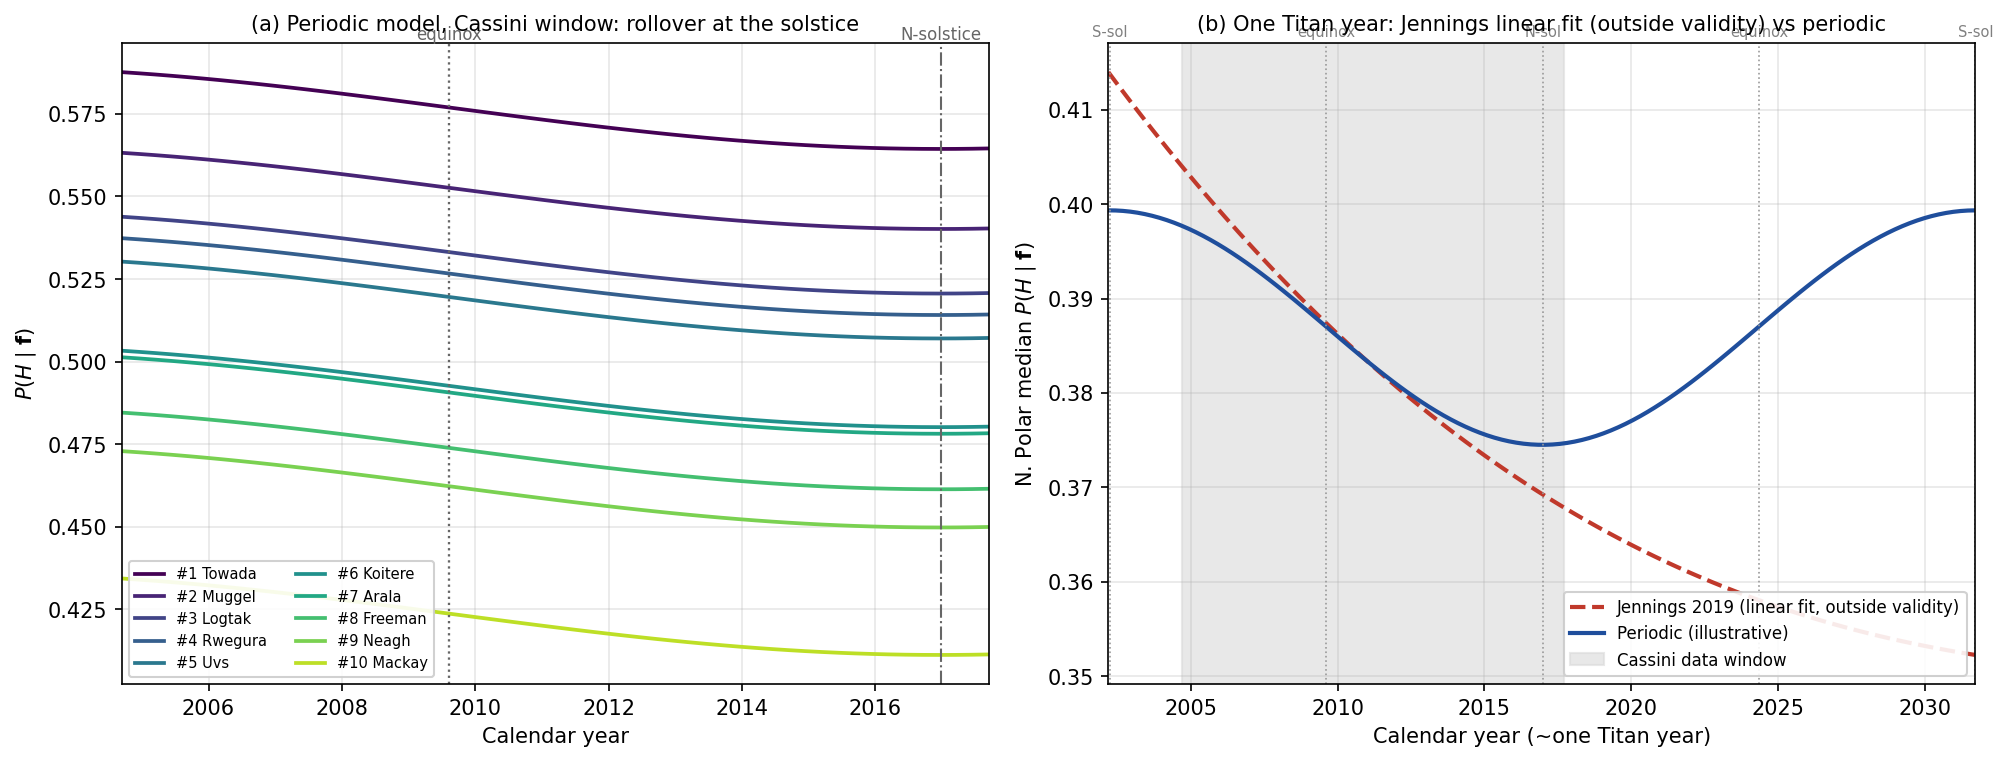
\includegraphics[width=\textwidth]{images/seasonal_ph_periodic.png}
  \caption{Illustrative comparison of the \citet{Jennings2019} linear-in-year
    temperature model (valid only over the Cassini window $Y \in [-4.9,
    +8.1]$) with a periodic model that substitutes the true astronomical
    subsolar latitude $26.7\textdegree \cdot
    \sin(2\pi(\text{year}-2009.61)/29.46)$ into the same cosine form, with
    amplitude and contrast held at equinox values.  (a)~Across the Cassini
    window the top-10 site curves roll over near the 2017 northern summer
    solstice.  (b)~Over a full Titan year the periodic model (solid) is
    bounded and repeats with the $29.46$\,yr period, whereas the linear fit
    (dashed) cannot be extrapolated past the shaded data window.  The periodic
    model is illustrative and is not fit to or validated against data.}
  \label{fig:seasonal_periodic_app}
\end{figure}

\section{Summary}
\label{sec:seasonal_summary}

Within the present framework, \titan{}'s surface habitability is seasonally
robust: only the methane cycle feature shows measurable modulation across half
a Titan year (one equinox, with the solstice reached only at the mission's
end), and even that modulation ($\leq 0.04$ in $P(H)$) leaves every site
ranking intact.  The framework can therefore be used for seasonal questions,
but the present result should be read as a directional, illustrative trend
rather than a validated seasonal climatology.  A full seasonal treatment is
left as future work (Section~\ref{sec:future_work}): it would incorporate
time-resolved lake extents for $f_1$, shoreline change for $f_5$, and a
validated periodic temperature model in place of the window-limited
\citet{Jennings2019} linear fit.
